\chapter{Implementation of the Game}
``Space-run'' was developed using the Godot Engine (version v3.2.3.stable), an open-source game engine licensed under the MIT License. It is a cross-platform tool that offers a range of features for game development, including a visual scripting language, 2D and 3D graphics support, and a powerful physics engine. The Godot Engine utilizes a node-based architecture, where nodes are organized within scenes that can be reused, instanced, inherited, and nested. This structure allows for efficient project management and development within the engine. The game was written entirely in GDScript, the primary scripting language of the Godot Engine (\cite{GodotDocs}).

In addition to using the Godot Engine, I also utilized Blender (version 6.2.0) (\cite{blender}) for creating and animating the characters in the game. Blender is popular open-source 3D modeling and animation software that offers a range of features for creating detailed and realistic characters. The characters were then imported into the Godot Engine using the .glTF 2.0 \cite{gltf} file format, which is a widely supported file format for exchanging 3D graphics data.

The game can be run on any platform provided within the Godot engine, and its source code, and the source code for the whole thesis can be found online (\cite{spacerunai}).

\section{The top-level organization}
\begin{figure}[h]
    \centering
    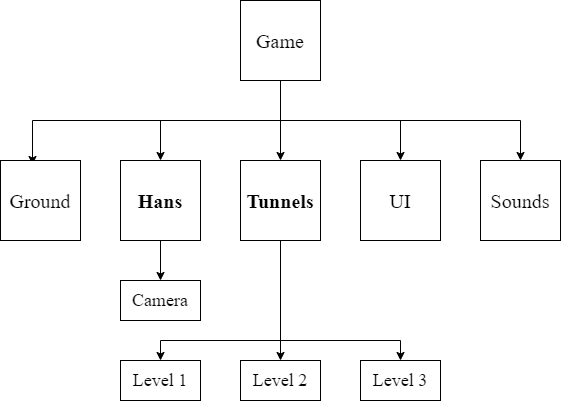
\includegraphics[width=0.8\textwidth]{game_tree}
    \caption{Structure of Game.tscn}
    \label{fig:game_tree}
\end{figure}

The main scene for the game, referred to as \texttt{Game.tscn}, is depicted in Figure \ref{fig:game_tree}. It includes several nodes, including Ground, UI, Sounds, Game, Hans, and Tunnels. The Ground node is a CSGBox\footnote{A CSGBox is a 3D object that represents a box with a Constructive Solid Geometry (CSG) shape.} that serves as the ground in the game, while the UI and Sounds nodes handle the user interface and audio aspects, respectively. The Game, Hans, and Tunnels nodes contain the majority of the game's functionality. Specifically, the Game node manages the overall gameplay, the Hans node controls the player character, and the Tunnels node manages the movement and appearance of the tunnels.

For a more in-depth understanding, let us examine some of the core aspects of the game in the following sections.

\section{Game}
The script for the Game node is the initial point of the game session and includes both the \texttt{\_start()} and \texttt{\_game\_over()} methods. It also serves as a link between the game and the agent environment described in Chapter \ref{agent_code_chapter}, and as such includes all of the necessary set methods for the agent environment. These methods allow for communication between the game and the agent environment, enabling the agent to interact with and influence the game.

The following text describes the core functionalities of the main methods within \texttt{Game.gd}:
\begin{itemize}
\item The \texttt{\_ready()} function is called at the start of the game's execution and, after setting up the environment, it triggers the \texttt{\_start()} function. This function initiates the gameplay and sets the necessary conditions for the game to proceed.
\item As described in more detail in Chapter \ref{agent_code_chapter}, the user can specify environment parameters and a starting level for the agent through the command line. These parameters determine the obstacles that the player will face and the starting position of the player character, Hans. The \texttt{\_start()} function incorporates these parameters into the obstacle arrays and positions Hans accordingly. The function also generates the obstacles for the designated starting level. The creation and deletion of obstacles during gameplay is discussed in Section \ref{tunnel_script} of this chapter.
\item The \texttt{\_game\_over} function manages the end of the game and sends a signal to the top-level script, \texttt{Main.gd} (described in Chapter \ref{agent_code_chapter}), indicating that the game has ended. It also provides \texttt{Main.gd} with the necessary information about the game's status and outcome.
\end{itemize}

\section{Hans}
The next node we want to examine is Hans. While \texttt{Hans.tscn} is a scene with the main character and its necessary animations, what interests us more is the \texttt{Hans.gd} and its key components.

\begin{center}
\line(1,0){400}
\begin{lstlisting}
func physics_Process(delta):
    tunnels.deleteObstacleUntilX(...)
    
    if translation.x < new_trap:
        createNewTrap()
        
    score._on_Meter_Passed() # update score
    
    velocity = Vector3.LEFT * speed
    velocity = moveAndSlide(velocity)
    
    checkCollisions()
    
    tunnels.bugVirusMovement(delta, curr_tunnel)
    
    if isShootingButtonPressed:
        shoot()
        
    state.updateState(...)
end
\end{lstlisting}
\line(1,0){400}
\end{center}

The primary function within \texttt{Hans.gd} is the \texttt{\_physics\_process()}, which is called on every tick of the game. It handles the main aspects of the player character through the use of various methods and functions. These include deleting passed obstacles, creating new obstacles every 50 meters, updating the score, handling the movement of the player character, bugs and viruses, and determining the current state of the player. The state label, which is displayed on the upper right corner of the screen (as shown in Figure \ref{fig:third_tunnel}), is the primary information that agents receive when making decisions about their next move, as described in Chapter \ref{agent_code_chapter}. The \texttt{\_physics\_process()} function also handles collisions and shooting if the player chooses to do so. Overall, this function plays a crucial role in the gameplay and management of the player character.

It is also worth noting that this script handles the movement of the tunnels to the back as Hans passes them, with the first tunnel being moved to be after the third one. This feature allows for the game to be infinite, as the tunnels are constantly cycled and reused.

\begin{figure}[h]
    \centering
    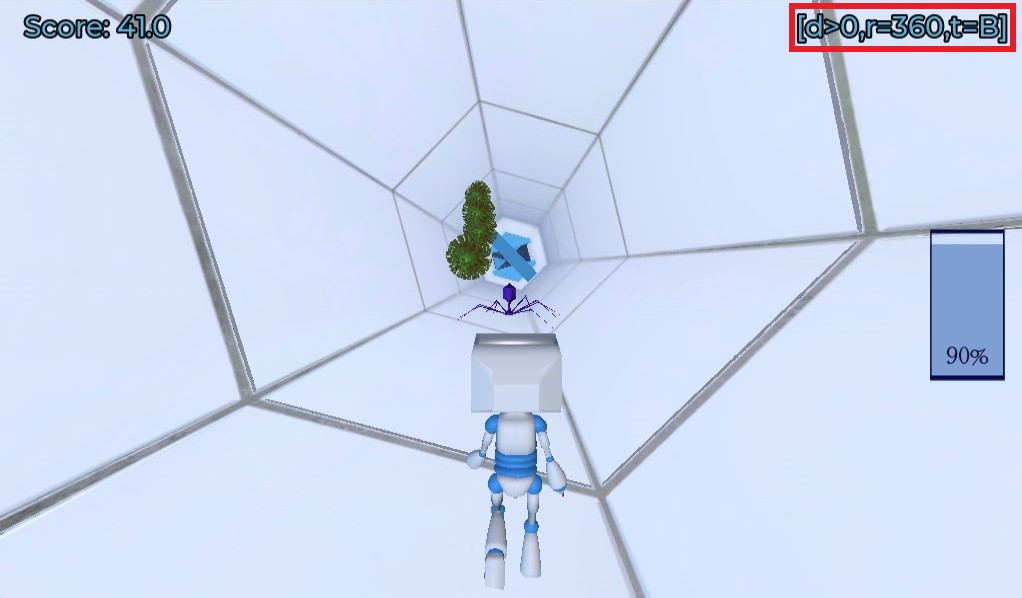
\includegraphics[width=\textwidth]{third_tunnel}
    \caption{State}
    \label{fig:third_tunnel}
\end{figure}

\section{Tunnels}
\label{tunnel_script}
The Tunnels node, which is a child of the main scene in the game tree, contains three child nodes of the Spatial type\footnote{A Spatial node is a type of node that represents a 3D object or transformation in the game world. It is a versatile node that can be used to create and manipulate 3D objects, including meshes, materials, and lighting. Spatial nodes are often used as the root node for 3D objects in a scene, and they can be nested inside other Spatial nodes to create hierarchical transformations.} (level1, level2, and level3) and each of these nodes includes a CSGTorus\footnote{ A CSGTorus node is a type of 3D object that represents a torus shape in the game world.} node, which represents the physical appearance of the tunnels. Obstacles are added to the appropriate level node as instances. The \texttt{Tunnels.gd} script, which is attached to the Tunnels node, handles many of the previously mentioned functions such as obstacle creation and deletion and tunnel rotation. In the following code snippets, we will examine the \texttt{Tunnels.gd} script in greater detail.

\begin{center}
\line(1,0){400}
\begin{lstlisting}
func physics_process(delta):
    var move = game.agent.move(...)
    if move[0] == 1:
        tunnel = get_child(hans.get_current_tunnel())
        tunnel.rotate_object_local(Vector3.RIGHT, -ROTATE_SPEED * delta)
    elif move[0] == -1:
        tunnel = get_child(hans.get_current_tunnel())
        tunnel.rotate_object_local(Vector3.LEFT, -ROTATE_SPEED * delta)

    if hans != null: # If it is not instanced we can't call the function
        hans.switch_animation(move[1] == 1) # Shoot if necessary
end
\end{lstlisting}
\line(1,0){400}
\end{center}

The \texttt{\_physics\_process()} function within the \texttt{Tunnels.gd} script serves as the primary connection between the agent and the game. As shown in the provided code, the function retrieves the next move from the agent and rotates the tunnel accordingly, potentially including shooting as well. It should be noted that, in the case of the \texttt{Keyboard} agent, function move returns users input from the keyboard.

\begin{center}
\line(1,0){400}
\begin{lstlisting}
func create_first_level_traps(tunnel):
	var level = tunnel
	var num_of_traps = rand_range(MIN_TRAPS_PER_TUBE, MAX_TRAPS_PER_TUBE)
	x = position of the first trap
	
	for n in range(num_of_traps):
		# update x positon
		x -= rand.randi_range(TRAP_RANGE_FROM,TRAP_RANGE_TO)
		if x is outside the tunnel:
			break
		create_one_obstacle(level, x)
\end{lstlisting}
\line(1,0){400}
\end{center}

The function depicted in the code above serves to generate obstacles in the starting tunnel. By periodically creating traps in the tunnel ahead, the game is able to prevent lag caused by an excessive number of objects existing simultaneously. For that reason, this function is used only once, at the beginning of the game.

\begin{center}
\line(1,0){400}
\begin{lstlisting}
func CreateOneObstacle(level, x):
	var scene = pick_which_kind_of_obstacle_will_be_added
	var tunnel = get_the_level_we_are_making_traps_for
	var i = randomly_pick_an_obstacle
	
	# make an instance
	var obstacle = scene[i].instance()
	obstacle.translation.x = x
	
	tunnel.add_child(obstacle)
    rotate_obstacle(obstacle)
\end{lstlisting}
\line(1,0){400}
\end{center}

The tunnels are positioned along the x axis, and this function allows for the creation of obstacles within them at specific x positions and a random rotation.

\begin{center}
\line(1,0){400}
\begin{lstlisting}
func delete_obstacle_until_x(level, x):
	var tunnel = get_current_tunnel()
	for obstacle in tunnel.get_children():
		if obstacle is an obstacle type:
			if obstacle.translation.x > x:
				obstacle.queue_free()
			else:
				return
\end{lstlisting}
\line(1,0){400}
\end{center}

As previously mentioned, by dynamically deleting passed obstacles, the game is able to maintain a stable performance and avoid overloading the system.